\section*{Question 1}
\begin{enumerate}[label=(\alph*)]
\item
The optimal way to move the cranes between old and new sites can be found using the Hungarian method. The setup of the Hungarian method and initial two steps are shown in Figure~\ref{fig:q1_initial}. After the first two steps, optimality is not reached, therefore we find an improved solution in Figure~\ref{fig:q1_answer} which we discover is an optimal solution. The optimal solution for returning the four cranes to the new sites is shown in Table~\ref{tab:q1}.

\begin{figure}[htp]
\centering
\caption{\label{fig:q1_initial}Hungarian Method Setup}
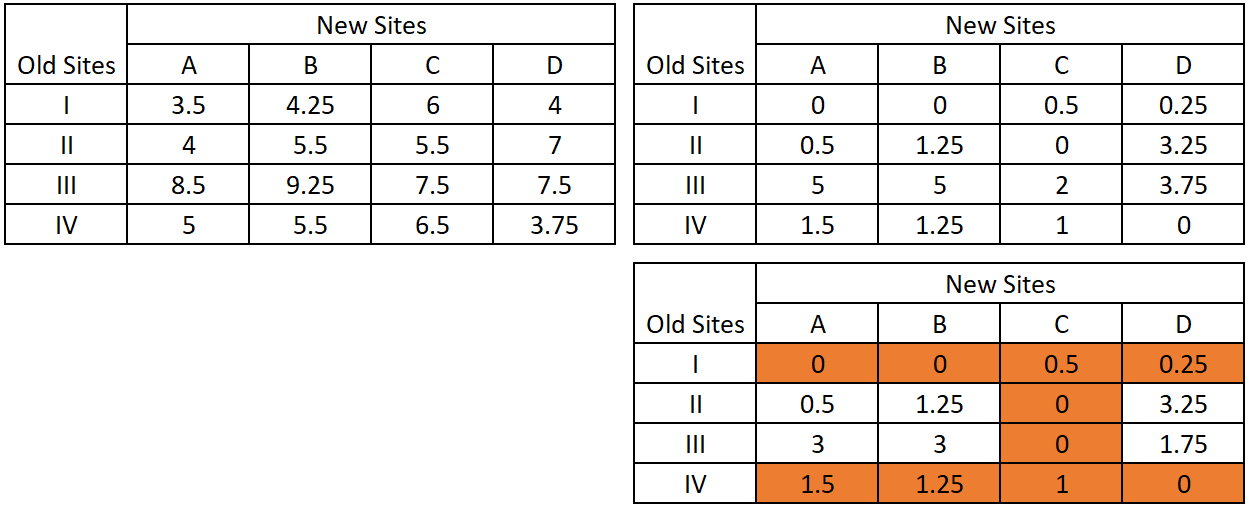
\includegraphics[width=\textwidth]{q1_setup.png}
\end{figure}

\begin{figure}[htp]
\centering
\caption{\label{fig:q1_answer}Hungarian Method Optimal Solution}
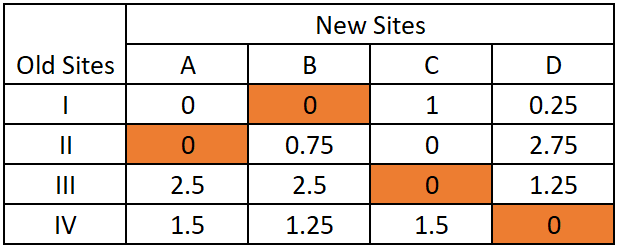
\includegraphics[width=0.59\textwidth]{q1_solution.png}
\end{figure}

\begin{table}[htp]
\centering
\caption{\label{tab:q1}Optimal Solution}
\begin{tabular}{|l|l|}
	\hline
	Old Sites	& New Sites	\\ \hline
	I			& B			\\ \hline
	II			& A			\\ \hline
	III			& C			\\ \hline
	IV			& D			\\ \hline
\end{tabular}
\end{table}
\clearpage

\item
The solution is confirmed using Excel Solver in Microsoft Excel. The solution was found to be the same, as seen in Figure~\ref{fig:q1_excel}. The Excel spreadsheet is included with the assignment submission as \texttt{question1.xlsx}.

\begin{figure}[htp]
\centering
\caption{\label{fig:q1_excel}Microsoft Excel Solution}
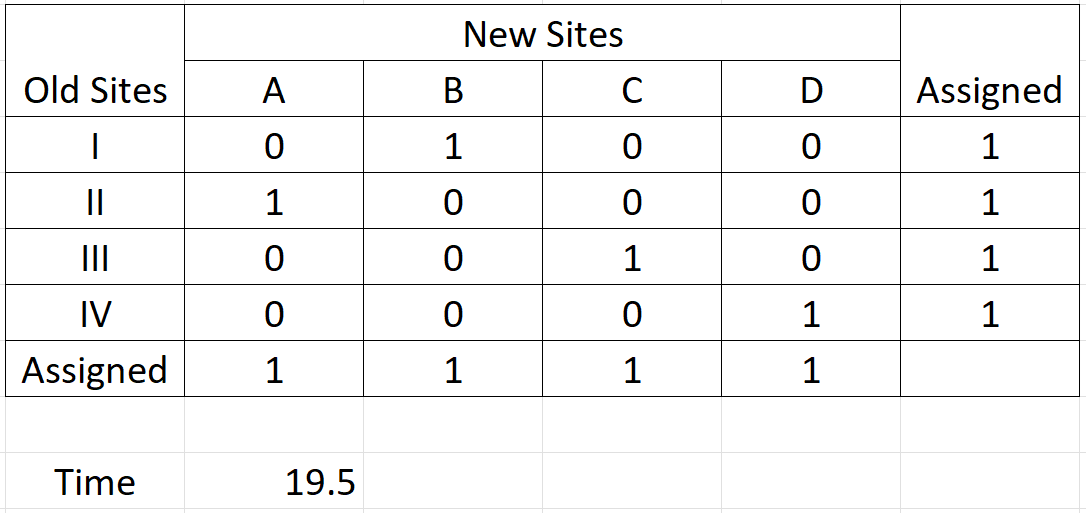
\includegraphics[width=\textwidth]{q1_excel.png}
\end{figure}

\end{enumerate}